

\chapter{L'évolution des êtres vivants}\label{ch:evolnat}

\lettrine[lines=2]{L}{'objectif} de ce chapitre est d'essayer de présenter la théorie de l'évolution, sa structure, les problèmes qu'elle a pu et qu'elle peut soulever ainsi que différentes façon de l'aborder.

Pour atteindre cet objectif nous allons d'abord retracer grossièrement l'histoire de cette théorie, en insistant sur la façon dont Darwin l'a énoncée et structurée, les problèmes que cette structure engendre et les outils déployés pour y répondre, que ce soit par Darwin lui-même ou par ses opposants et ses successeurs. Nous nous appuierons en grande partie sur les travaux de \cite{gayon1991darwinetlapresdarwin} et terminerons cette première partie en décrivant brièvement le consensus auquel ont abouti les recherches du XXe siècle dans le domaine. 

Dans un second temps nous essayerons de dégager quelques points que les travaux des successeurs de Darwin n'ont pas résolus, afin de montrer que de nombreuses questions restent en suspens et qu'y répondre demande une attention toute particulière. Pour illustrer ce constat nous nous attarderons sur le débat à propos des unités et niveaux de sélection. Ce débat sera un bon moyen d'introduire les problèmes actuels posés par l'étude de la théorie de l'évolution et les différentes approches envisagées pour y répondre. Nous terminerons en présentant une de ces approches plus en détail, celle de \cite{godfrey2009darwinian}.

\section{Histoire et principes de la théorie de l'évolution}\label{sec:cmpdr}

En 1859, Charles Darwin proposait une théorie pour essayer de rendre compte de la diversité des êtres vivants dans son livre l'Origine des Espèces\nocite{darwin1859originspeciesbymeansnaturalselectionorpreservationfavouredracesstrugglelife}. Pour lui cette théorie se résumait comme:
\begin{quote}
	%%Theory of descent with modification by variation and Natural Selection.
	Une théorie de la descendance avec modification par la variation et par la Sélection Naturelle.\\
	\citep[dernière édition, trad. \cite{gayon1991darwinetlapresdarwin}]{darwin1859originspeciesbymeansnaturalselectionorpreservationfavouredracesstrugglelife}.
\end{quote}
et fut ensuite plus couramment appelée la \emph{théorie de l'évolution par Sélection Naturelle}.

Pour bâtir cette théorie, \cite{gayon1991darwinetlapresdarwin} nous explique que Darwin propose et admet deux mécanismes:
\begin{itemize}
	\item L'hypothèse de la Sélection Naturelle: autrement dit <<\,la survie du plus apte\,>>.
	\item La descendance avec variation, autrement dit <<\,l'hérédité des différences individuelles\,>> \citep{gayon1991darwinetlapresdarwin}.
\end{itemize}

L'admission de ces hypothèses, et donc de la théorie qui en découle, permet de rendre compte de: l'évolution des espèces dans le temps (avec chez Darwin une notion de <<\,progression\,>>, <<\,d'amélioration\,>> des espèces) et de leur divergence les unes des autres. Mais cette théorie (et les hypothèses qu'elle présuppose), de par sa structure et son contenu, n'est simple ni à observer ni à démontrer. Surmonter ces difficultés et essayer de convaincre du bien fondé de ces théories fut l'une des tâches principales de Darwin, qu'il mena dans ses livres depuis l'Origine des Espèces jusqu'à ses derniers ouvrages. 

Nous verrons dans les parties qui suivent quelles étaient ces difficultés, en reprenant la structure de la théorie de l'évolution vue par \cite{gayon1991darwinetlapresdarwin} et en détaillant les deux points que nous avons dégagés plus haut. Nous verrons dans le même temps pourquoi Darwin ne réussit pas tout à fait à mener à bien sa tâche dans les sections \ref{sec:hered} et \ref{sec:SN}. Puis nous présenterons comment ses héritiers ont repri ses travaux pour essayer de terminer cette entreprise. Nous verrons à quels consensus les avancées faites dans la recherche en biologie et plus particulièrement sur la théorie de l'évolution ont abouti, et nous dirons deux mots de la Synthèse Moderne qui a en grande partie rendue possible ces consensus ainsi que sur \emph{la vision centrée sur le gène} (<<\,\emph{the gene eye view}\,>> en anglais) dans la section \ref{sec:SM}. 


\subsection{Descente avec modifications}\label{sec:hered}
Avant toute chose, et pour que la sélection Naturelle puisse agir et donc l'évolution selon Darwin avoir lieu, il faut que les caractères qui déterminent la fitness des individus (c'est à dire leur degré d'adaptation à leur environnement\footnote{La fitness est difficilement définissable en anglais et a fortiori en français. On parle souvent de \emph{valeur sélective} mais nous conserverons la plupart du temps le terme anglais de \emph{fitness}.}) soient \emph{transmis} à leurs descendants. Et non seulement ils doivent être transmis, mais pour qu'il y ait du changement, ils doivent aussi \emph{varier}. Or, ces variations et cette hérédité (la transmission), Darwin (il le concède lui-même) ne possède pas de théorie satisfaisante pour en rendre compte. Comment les parents transmettent-ils leurs caractères à leurs descendants et pourquoi ces caractères varient-ils, sont des phénomènes encore assez mal compris à l'époque. Néanmoins Darwin bâtit sa théorie de l'évolution en présupposant un certain type de transmission et un certain type de variations très précis. Selon lui, pour que l'évolution ait lieu, il faut que les caractères transmis \emph{varient} de façon aléatoire et \emph{graduelle} chez les descendants. Par exemple: une population d'individus de taille $X$ aura des descendants avec des tailles comprises entre $X-n$ et $X+n$ qui varient de façon quasi continue entre $-n$ et $n$. Ce sont ces variations aléatoires et continues sur lesquelles la Sélection Naturelle va pouvoir agir.

Ainsi, et pour que sa théorie générale de l'évolution tienne la route, Darwin doit donc construire et accepter une théorie de l'hérédité qui présente les propriétés dont sa théorie de l'évolution à besoin et que nous venons de présenter. De plus cette théorie doit être conforme aux nombreuses observations qu'il a faites dans la nature. Dans l'Origine des espèces il fera l'hypothèse de l'existence d'une telle théorie, en considérant que les mécanismes qui présentent ces propriétés existent mais qu'ils restent à trouver et comprendre. Puis, dans \cite{darwin1868variation}, il développera sa propre théorie, en reprenant les anciens concepts de la \emph{pangénèse}\footnote{Dans la théorie de la pangénèse les individus accumulent dans leurs cellules germinales des particules (gémules) de l'ensemble des cellules de leur corps. Ces particules serviront à reconstruire un nouvel individu lors de la reproduction. Il est à noter qu'avec cette théorie, Darwin conserve le concept lamarckien de transmission des caractères acquis, puisque les gémules s'accumulent toute au long de la vie de l'individu, et sont donc susceptibles de transmettre les caractères acquis pendant cette vie.}. Mais l'adoption de ces propriétés comme centrales à l'évolution et d'une théorie de l'hérédité qui possède ce type de propriétés pose plusieurs problèmes.

Dans un premier temps des problèmes théoriques. Un des détracteurs de Darwin, Jenkin, soutiendra en l'illustrant mathématiquement qu'une sélection agissant sur des variations continues qui se mélangent lors de la reproduction ne pourra que stabiliser ces variations autour de valeurs moyennes et n'aboutira pas à l'apparition de nouvelles valeurs moyennes (de nouveaux phénotypes). Il soutiendra aussi que l'apparition ponctuelle de nouveaux caractères aura de forte chance de passer inaperçue, les caractères nouveaux seront statistiquement ``dilués'' au milieu des caractères existants et finiront par disparaître.

Ce sera pour Darwin la critique la plus sérieuse faite à sa théorie et il ne réussira pas vraiment à la surmonter. D'une part car elle est une conséquence directe des choix théoriques qu'il a fait vis-à-vis de l'hérédité et des variations qu'elle doit permettre, d'autre part car elle vient d'une personne dont l'approche scientifique est totalement différente de la sienne. En effet Jenkin est un ingénieur, beaucoup plus porté sur les mathématiques que Darwin, qui est plutôt un naturaliste classique, homme de terrain. Ceci rend à Darwin le défi adressé par Jenkin <<\,un défi auquel assurément sa culture et son expérience propre, fort peu quantitatives, ne lui permettaient pas de se mesurer\,>> \citet[p.~105]{gayon1991darwinetlapresdarwin}. Ainsi, même si les critiques de Jenkin ont souvent (et à juste titre) été qualifiées de <<\,pamphlet réactionnaire\,>>, elles ont eu le mérite de déplacer l'intérêt des scientifiques vers des problèmes théoriques profonds de la théorie de l'évolution. Cette critique a dressé un véritable <<\,cahier des charges [\ldots] aux théoriciens futurs\,>> (\emph{ibid.}), les invitant à proposer <<\,une description plus \emph{rigoureuse} de ce qu'ils appellent variations\,>> (\emph{ibid.} p.~103, emphase d'origine) et ouvrant la voie de <<\,bon nombre de thèmes caractéristiques de la future biométrie, et au-delà, de la génétique des populations\,>> (\emph{ibid.} p.~105).

Un second problème (non sans lien avec le précédent) que vont rencontrer les hypothèses de Darwin est celui, plus empirique cette fois, posé par la redécouverte des lois de Mendel au début du XXe siècle. En effet, quelques décennies après la disparition de Darwin, les biologistes cellulaires montreront, en s'appuyant sur un très grand nombre d'expériences, que si il y a bien une transmission héréditaire de certains caractères via ce qu'il sera convenu d'appeler les gènes, ces caractères ne varient pas de façon continue chez les descendants, mais sont des caractères discrets qui ne peuvent qu'être hybridés selon certaines lois statistiques régulières. Cette constatation, avait déjà été faite à l'époque de Darwin par Gregor Mendel, mais était alors passée inaperçue. D'après ces observations, les caractères transmis par hérédité ne peuvent pas véritablement se <<\,mélanger\,>>, ce qu'avait imaginé \cite{darwin1868variation} dans son livre <<\,De la variation des animaux et des plantes sous l'action de la domestication\,>> pour soutenir une théorie de l'hérédité en accord avec sa théorie de l'évolution. Les expériences des biologistes tranchaient: il n'y a pas de <<\,gémules\,>>. 

Ainsi non seulement, la théorie de la \emph{pangénèse} de Darwin était-elle fausse empiriquement, mais elle laissait place à une théorie génétique qui ne présente pas, à première vu, les propriétés nécessaires à l'évolution selon Darwin. Paradoxalement, c'est cette génétique qui offrira plus tard ces propriétés capables d'articuler correctement la théorie de l'hérédité avec la théorie de l'évolution pour permettre de résoudre les problèmes soulevés par Jenkin.

\subsection{Hypothèse de la Sélection Naturelle}\label{sec:SN}
Une fois une théorie de l'hérédité des variations individuelles admise (avec, comme nous venons de le voir, les problèmes que cela comporte), la sélection naturelle peut jouer son rôle. Nous résumerons l'action de cette Sélection Naturelle ainsi:
\begin{quote} Les individus avec les variations offrant à ceux qui les portent la meilleure adaptation (ie les individus qui possèdent la meilleure \emph{fitness}) vivrons plus longtemps et/ou laisserons en moyenne plus de descendants.\end{quote}

	Pour \citet[p.~22]{gayon1991darwinetlapresdarwin} c'est <<\,l'hypothèse organisatrice\,>> de la \emph{théorie} de Darwin. Mais Darwin ne possède aucun \emph{fait} la justifiant, aucune preuve directe de cette hypothèse. L'action de celle-ci n'est perceptible qu'à des échelles de temps géologiques difficiles à appréhender et encore moins observables par les humains. Pour arriver à convaincre, Darwin va donc devoir utiliser l'analogie avec la Sélection Artificielle.
	
	Cette analogie, sur laquelle nous reviendrons un peu plus tard pour des raisons différentes (section \ref{sec:cmpdr:sa}), s'appuie sur les très nombreuses études d'éleveurs que Darwin a beaucoup étudiées. Dans ces études les éleveurs expliquent comment ils sont capables de transformer et faire diverger de beaucoup les espèces domestiques en sélectionnant certains spécimens particuliers qui présentent certains critères qui intéressent les éleveurs. 
	
	Pour Darwin, si les êtres humains, en appliquant ce genre de pression sélective explicite et directe, peuvent modifier les espèces vivantes domestiques, alors il doit exister une force analogue capable de modifier les espèces dans la nature. Une force qui pourrait rendre compte de la diversité et des adaptations de ces espèces. Cette force, qui agirait sur des variations transmises par hérédité comme nous l'avons vu et défini ci-dessus (section \ref{sec:hered}), Darwin l'appelle la Sélection Naturelle. Grossièrement résumé par nous il la décrit ainsi: les individus les mieux adaptés se reproduiront plus et auront plus de descendants dans les générations suivantes. 

	Il est intéressant de noter, car nous y reviendrons, qu'en définissant cette Sélection Naturelle Darwin insiste sur une propriété importante pour lui. Les variations qui vont, ou non, augmenter les chances de survie et de reproduction (la \emph{fitness}) doivent être portées par les individus (individus qu'il identifie aux <<\,organismes biologiques\,>>, identité dont nous reparlerons). Pourtant, que l'\emph{individu} soit porteur des variations nécessaires à l'évolution n'est pas si évident qu'il n'y paraît. À l'époque déjà, Wallace, co-<<\,découvreur\,>> de la théorie de l'évolution par sélection naturelle, avançait que les variations étaient des différences entre des populations d'individus, et que la sélection portait sur ces populations, et non sur les individus qui les composent. Ce problème, qui préfigure les questions des unités de sélection, est un problème toujours d'actualité et nous reviendrons plus amplement dessus dans la section \ref{sec:lvl}. 

Mais qu'importe pour le moment cette querelle et le niveau sur lequel peut opérer la sélection. Il n'en demeure pas moins qu'à l'époque, ni Darwin ni Wallace ne pouvaient prouver cette hypothèse de la sélection naturelle. Trouver cette preuve fera partie du legs de Darwin à ses successeurs et cette lacune n'aura de cesse d'être pointée du doigt par ses détracteurs. Il faudra attendre quelques dizaines d'années et les biométriciens, pour que soient entreprises les premières tentatives visant à démontrer empiriquement l'action de la Sélection Naturelle.

Ce sont les nouvelles méthodes statistiques, apportées par Galton, puis Pearson et Weldon, qui vont proposer ce qui se rapprocherait le plus des premières preuves mathématiques et empiriques de l'action de la Sélection Naturelle. Le développement de ces méthodes va fortement influencer toute la biologie de l'évolution pendant presque 50 ans, jusqu'à la création de la génétique des populations dont nous reparlerons plus tard; et leur introduction doit beaucoup aux critiques de Jenkin auxquelles les biométriciens vont essayer de répondre.

En effet, dans ce désir de répondre à Jenkin et proposer un preuve de la Sélection Naturelle, Pearson et Weldon, deux acteurs majeurs au sein de l'école biométrique, vont mettre au point tout un ensemble de techniques pour essayer de rendre compte des effets de la Sélection Naturelle. Ils s'inspireront des travaux sur les distributions normales et les corrélations de caractères morphologiques de Francis Galton ---un cousin de Darwin considéré comme un des pères fondateurs de l'eugénisme--- pour montrer que: les conditions de variation nécessaires à l'action de la Sélection Naturelle comme la pensait Darwin sont présentes dans la nature, et que l'action même de cette Sélection Naturelle, sous réserve d'utiliser les outils adéquat, peut être visualisée. 

Dans une série de publications datant du début des années 1890 (voir par exemple: \cite{weldon1893certaincorrelatedvariationsincrangonvulgaris}), ils montreront, en s'appuyant sur les analyses statistiques de très haut niveau de Pearson et sur les minutieux et rigoureux relevés morphologiques de Weldon, ce qu'ils considèrent comme \emph{l'effet de la sélection naturelle} sur des populations de crabes. Pour ça ils vont devoir mettre au point certains tests statistiques dérivés de ceux de Galton pour: 
\begin{enumerate}
	\item Montrer que deux populations de crabes ne présentent pas de différences morphologiques d'un point de vue statistique et ont donc toutes les raisons d'être deux populations de la même espèce, à un détail près qu'ils vont illustrer dans le suite de l'étude.
	\item Montrer qu'une des deux populations, pour un caractère morphologique particulier, présente un dimorphisme que les auteurs mettent à jour statistiquement (autrement dit: pour ce caractère précis les variations ne sont pas réparties de façon normale autour de la moyenne mais sont en fait réparties comme la somme de deux distributions normales autours de deux moyennes statistiquement différentes).
\end{enumerate}

Néanmoins ces résultats ne répondent pas directement aux critiques formulées par Jenkin. Si ils montrent que la sélection peut agir au niveau des individus et faire se déplacer certains caractères morphologiques, ils ne démontrent pas pour autant que les espèces peuvent durablement se modifier par ce biais et diverger véritablement. D'où les arguments de l'époque, avancés par les <<\,mutationistes\,>>. Ces derniers, reprenant certains arguments de Jenkin (et aussi de Galton, ce qui est assez ironique compte tenu du faite que Weldon et Pearson aussi reprennent beaucoup d'outils galtonniens) continueront d'avancer que la sélection telle que décrite par Darwin ne peut que faire dévier les caractères morphologiques autours de moyennes constantes, fixes. Les traits phénotypiques des individus sont en réalité, contrôlés par des <<\,atomes\,>> discrets, qui restent les mêmes dans l'histoire évolutive de l'espèce. Les changements ne peuvent être apportés que par des mutations brutales et importantes qui vont modifier ces atomes et transformer les caractères morphologiques. Ces critiques seront d'autant plus fortes et la position des biométriciens d'autant plus difficile à tenir que la redécouverte des lois de Mendel offrira aux mutationistes l'appui empirique dont n'a jamais jouit la théorie <<\,gradualiste\,>> envisagée par Darwin.

\subsection{Théorie synthétique de l'évolution}\label{sec:SM}
Au début du XXe siècle la théorie de l'évolution affronte donc un problème. D'un côté Weldon et Pearson semblent démontrer statistiquement et empiriquement qu'une certaine évolution s'appuyant sur des variations graduelles est possible, d'un autre côté les études empiriques montrent que ces variations graduelles n'apparaissent que rarement voire pas du tout dans la nature, et qu'en réalité il n'y a que des caractères discrets qui s'hybrident selon les lois de Mendel. Par conséquent, pour les partisans de ce \emph{mendélisme}, la sélection naturelle de caractères qui varient de façon continue (ce qu'avait défini Darwin) ne peut pas faire évoluer les espèces. Ce sont, comme nous venons de le dire, les mutations ponctuelles de caractères discrets qui doivent être à <<\,l'origine des espèces\,>>. 

Mais la donne va progressivement changer. En 1918, Fisher, dans un article central en génétique des populations \citep{fisher1918thecorrelationbetweenrelativesonthesuppositionofmendelianinheritance}, démontre que le \emph{gradualisme} nécessaire à la sélection naturelle de Darwin n'est pas incompatible avec des caractères mendéliens. C'est ainsi qu'avec Wright et Haldane ils vont, pendant la décennie suivante, réconcilier théoriquement et mathématiquement la ségrégation de caractères discrets de Mendel avec la sélection de caractères aux variations continues de Darwin. 

Cette réconciliation mathématique s'avèrera au final une aubaine pour le darwinisme. Elle va offrir à ce dernier la théorie de l'hérédité qui faisait défaut à Darwin: la théorie génétique de l'hérédité mendélienne.

Suite à quoi s'en suivirent, entre 1930 et 1960, plusieurs décennies de <<\,synthèse\,>>, au cours desquelles les différents domaines de la biologie vont être rattachés empiriquement et théoriquement à cette théorie de l'évolution <<\,réconciliée\,>>. Que ce soit en paléontologie, en écologie, en botanique, en génétique ou en zoologie, de nombreux livres parurent, pièces aujourd'hui centrales dans chacun de ces domaines, pour faire le lien entre la nouvelle biologie moderne de l'évolution et les différentes disciplines impliquées.

Cette période, et le paradigme scientifique qui en découla et dont nous avons déjà dit quelques mots en introduction, furent appelés la synthèse moderne (SM, souvent aussi appelée théorie synthétique de l'évolution, TSE, dans la littérature francophone) d'après le livre d'un de ses artisans: \cite{huxley1942evolution}. 

Elle fut témoin de nombreuses avancées et a eu (et a toujours) un impact profond sur la biologie dans toute sa diversité. Nous ne rentrerons pas dans les multiples détails de cette riche époque. Néanmoins il convient d'en dire quelques mots, car à la fin de ces années de synthèse un certain consensus sur l'interprétation des phénomènes évolutifs a émergé. Or ce consensus aura une influence directe sur les méthodes utilisées en Robotique \'Evolutionnaire et sur l'approche biologique qui l'inspire. Il n'est donc pas inutile d'essayer de saisir \emph{comment est apparu} et \emph{quel est} ce consensus.

Les généticiens des populations (Fisher, Haldane, Wright\ldots) en réconciliant Mendel et Darwin, ont remis le support de l'hérédité, le gène, au centre des recherches sur l'évolution. Fisher lui-même explique l'évolution comme des variations de \emph{fitness} sur des variations de fréquences génétiques \citep{fisher1930geneticaltheorynaturalselection}.
Il devenait ainsi possible de résumer l'évolution des êtres vivants à l'évolution de leur bagage génétique. Mieux encore, avec la découverte de l'ADN dans les années 50 le rêve réductionniste de la science moderne semblait accessible à la théorie de l'évolution. En effet, pour étudier cette dernière il suffit d'étudier des variations de fréquences de gènes. Or les gènes sont portés par l'ADN, une molécule dont on peut théoriquement comprendre les propriétés chimiques, il suffit donc d'étudier les propriétés physico-chimiques de cette molécule pour comprendre l'évolution.

La force heuristique de cette idée réductionniste, qui avance que comprendre l'évolution des gènes peut aider à comprendre l'évolution des êtres vivants, a probablement été un élément clef du succès de la synthèse moderne. Elle fut d'autant plus vite adoptée qu'elle présentait une structure, comme le souligne \cite{griesemer2002whatisepiaboutepigenetics}, isomorphe avec un schéma de l'évolution très influent au début du siècle: le weismannisme. 

Weisman avait en effet montré, dans l'optique d'éliminer les réminiscences lamarckiennes de la théorie de l'évolution du début du XXe, que seules les variations présentes dans les cellules germinales sont importantes. Les autres cellules de l'organisme, les cellules somatiques, n'ont pas de rôle évolutif particulier puisque les modifications qu'elles peuvent subir ne sont pas transmises à la descendance. Il y a donc selon lui, une barrière entre la lignée des cellules germinales (le germen), qui sont transmises de génération en génération, et qui peuvent évoluer, et les cellules somatiques (le soma), qui ne sont que le produit de l'information contenue dans les cellules germinales et qui n'évoluent pas. Cette barrière est conceptuellement la même que celle faite par la synthèse moderne entre le génotype, dont les variations sont transmises de génération en génération, et le phénotype, l'expression de ce génotype, dont les variations ne sont pas transmises. La transition de l'une à l'autre allait donc de soi.

L'unidirectionnalité de cette barrière (l'information va du germen vers le soma, du génotype vers le phénotype, mais pas dans l'autre sens), qui permet le réductionnisme décrit plus haut, fut encore renforcée par l'établissement dans les années 70 du dogme centrale, proposé dans la lignée de Crick, par Jacob et Monod. Avec le dogme central la cellule, le phénotype, s'avérait bien le produit <<\,chimique\,>> d'une traduction du génome, irréversible, avec un sens (ADN$\rightarrow$transcription$\rightarrow$traduction$\rightarrow$protéine) donné et unidirectionnel.

Le gènes sont ainsi devenus les agents principaux de l'évolution, la cellule n'était plus qu'un <<\,véhicule\,>> \citep{dawkins76selfishgene} pour les transporter. On pouvait résumer l'histoire évolutive des êtres vivants à l'histoire évolutive des gènes qui les composent. C'est <<\,\emph{the gene eye view}\,>>, comme fut baptisée cette vision de l'évolution. En tant que schéma cohérent elle fut d'abord proposée par \cite{williams1966adaptationandnaturalselection} puis popularisée par \cite{dawkins76selfishgene}. Sa remarquable force explicative, sa simplicité et sa puissance réductionniste lui ont très vite assuré un certain succès non seulement dans la communauté scientifique mais aussi auprès du grand public.

Ainsi, quand à la fin des années 60 la synthèse moderne se terminait et entrait dans sa phase <<\,institutionnelle\,>>, la <<\,\emph{gene eye view}\,>> s'installait comme un élément central de celle-ci. En devenant le paradigme enseigné et adopté par tous, la SM a ancré au sein de la communauté scientifique au sens large (et plus seulement parmi les biologistes) les idées et concepts qu'elle avait mis près d'un demi-siècle à établir. Inévitablement donc, fut diffusée et adoptée cette vision, indissociable de la SM, d'un organisme réductible à l'information génétiques qui le compose. Cette information génétique est porteuse des variations nécessaires à l'évolution et va les reproduire et les transmettre de génération en génération. C'est elle la cible de cette évolution. 

C'est cette vision qui va offrir le schéma parfait que vont pouvoir reprendre les informaticiens pour réaliser les intuitions de Turing. Sa simplicité et son efficacité, alliées à de solides modèles théoriques et mathématiques, vont permettre aux informaticiens de la reprendre telle quelle pour développer l'Algorithmique Évolutionnaire puis plus tard, la Robotique \'Evolutionnaire. 

Mais la synthèse moderne et la <<~\emph{gene eye view}~>> n'ont pas résolu tous les problèmes théoriques soulevés par les propositions de Darwin pour autant. Nous allons voir comment ceux-ci sont réapparus et ont été repris par les scientifiques et philosophes depuis les années 1970.


\section{Problèmes et réflexions actuels sur la théorie de l'évolution}\label{sec:pbm}
\subsection{Niveaux et unités de sélection}\label{sec:lvl}
Dans la section \ref{sec:SN} nous avons dit que, pour peu qu'ils transmettent leurs caractères à leurs descendants et que ces caractères varient, les <<\,individus\,>> les mieux adaptés vivront plus longtemps et auront plus de descendants. Ainsi, génération après génération, les populations se verront composées de plus en plus d'individus mieux adaptés, les caractères divergeront, les espèces évolueront. Nous avons vu que cette définition a posé quelques problèmes quant à la nature des variations nécessaires, problèmes qui furent partiellement résolus par la synthèse moderne et la réconciliation du mendélisme avec Darwin. Mais la théorie de Darwin soulève d'autres questions. Dans un article majeur sur le sujet, \cite{lewontin70unitsselection} reprend cette théorie pour la formuler et la résumer dans des termes plus actuels de la façon suivante:
\begin{enumerate}
	\item Dans une population des individus différents ont une morphologie, une physiologie et des comportements différents (\emph{variation phénotypique}).
\item Des phénotypes différents ont des taux de survie et de reproduction différents dans des environnements différents (\emph{fitness différentielle}).
	\item Il y a une corrélation entre parents et descendants à chaque génération future (\emph{hérédité de la fitness}).
\end{enumerate}

L'auteur explique que le niveau d'abstraction de cette définition n'impose pas l'organisme comme <<\,individu\,>>. N'importe quelle entité répondant aux trois critères que Lewontin énonce peut remplir ce rôle d'individu. Pour lui cette définition s'applique très bien aux différents niveaux d'organisation biologique. Les <<\,individus\,>> peuvent aussi bien être les cellules, les chromosomes, les gènes, les organes au sein d'un organisme, les organismes entre eux ou même les espèces d'organismes entres elles. 

Déjà à l'époque de Darwin et comme nous l'avons brièvement évoqué, Wallace considérait que les populations et non les individus étaient sélectionnés, suggérant ainsi que la sélection pouvait agir à différents niveaux que celui envisagé par Darwin. Et en réalité, même si pour ce dernier, la pression de sélection ne peut porter que sur les variations des individus (individus qui sont pour lui des organismes multicellulaires), il considérera dans son livre \emph{The descent of man} \citep{darwin1871thedescentofman}, que les sociétés humaines (donc des \emph{populations} d'individus biologiques) peuvent être soumises à une force similaire à la sélection naturelle qu'il avait initialement définie pour les organismes. Un peu plus tard, Weismann, dont nous avons déjà parlé pour ses travaux sur le germen et le soma, fut aussi un de ceux qui théorisa beaucoup cette idée que des populations peuvent être sélectionnées.

Ainsi la question de savoir quelles sont les \emph{unités} et à quels \emph{niveaux} d'organisation biologique agit la sélection naturelle est une question aussi vieille que la théorie de l'évolution elle-même. Aujourd'hui désigné comme le débat sur les <<\,unités et niveaux de sélection\,>>, ces réflexions ont connu un regain d'intérêt important à la suite de l'article de Lewontin. La crise du mendélisme était passée et la synthèse moderne avait fini d'offrir un cadre stable et un ensemble de théories et de modèles cohérents pour pouvoir réfléchir à nouveau sur ces problèmes. L'attrait pour ces questions repris d'autant plus vigoureusement qu'au sortir de la synthèse moderne était adopté, comme nous l'avons souligné dans la partie précédente, le consensus du <<\,\emph{gene eye view}\,>>, qui prend un parti très tranché sur ces questions des niveaux de sélection: la sélection agit sur les gènes et rien d'autre. 

Nous avons vu dans la section \ref{sec:SM} les apports et intérêts de cette vision mais elle fut néanmoins très vite l'objet de nombreuses critiques. \cite{wimsatt1980theunitsofselectionandthestructureofthemultilevelgenome}, par exemple, remettra en cause la vision de \cite{williams1966adaptationandnaturalselection} (et de \cite{dawkins76selfishgene}), en argumentant qu'elle ne peut rendre compte de tous les phénomènes évolutifs en biologie. Pour lui la fitness des individus n'est pas réductible à la fitness des gènes qu'il possède, ces derniers interagissent de façon trop complexe et non linéaire entre eux. \cite{gould2002thestructureofevolutionarytheory} écrira même, dans l'imposante synthèse de sa réflexion qu'est <<\,La Structure de la Théorie de l'\'Evolution\,>>, que:
\begin{quote}
	[\ldots] la théorie de l'évolution centrée sur le gène était indéfendable.\\ \citep[p.~855]{gould2002thestructureofevolutionarytheory}
\end{quote}
Ces problèmes et visions divergentes sont nombreux et, comme l'écrit Gould dans le même ouvrage,
\begin{quote}
	[o]n pourrait organiser la discussion sur ce sujet très difficile et très important d'une centaine de façons différentes. (\emph{ibid.}, p.~833).
\end{quote}
Il est donc difficile d'en faire une revue exhaustive. \cite{lloyd12unitsandlevelsofselection}, dans son article qui essaye justement de faire cette analyse complète de la littérature, considère qu'en réalité il serait plus judicieux de décomposer ce problème en quatre questions différentes qui sont en général mélangées dans la littérature sur le sujet. Pour elle l'important est de dégager: 
\begin{enumerate}
	\item quelles unités sont sélectionnées,
	\item à quel(s) niveau(x) se situent ces unités,
	\item qui bénéficie des évolutions produites par la sélection et
	\item où se manifestent les adaptations acquises.
\end{enumerate}

Analyser et dégager ces axes est une chose complexe  et nous ne le ferons pas ici.  Nous nous contenterons de considérer les 4 points ensembles sous le nom <<\,niveaux et unités de sélection\,>>. En revanche, pour illustrer comment et pourquoi ce débat a pu diviser et continue de mobiliser presque tous les biologistes contemporains, nous allons présenter quelques arguments et quelques pistes de réflexions qu'ont pu avancer certains chercheurs et philosophes depuis une quarantaine d'années.

Une des approches la plus reprise et admise depuis les années 60, puisqu'elle apporte en quelque sorte la réponse directe de la <<\,\emph{gene eye view}\,>> à ces questions, est l'approche de \cite{dawkins76selfishgene} et \cite{hull1974philosophyofbiologicalscience}. Pour clarifier le débat, ces deux auteurs proposent de distinguer les \emph{interacteurs} (les \emph{véhicules} pour \cite{dawkins76selfishgene}), qui agissent dans l'environnement et interagissent entre eux, des \emph{réplicateurs}, qui se répliquent de génération en génération. Cette séparation offre, surtout à Dawkins, le moyen de construire une théorie de la Sélection Naturelle en accord parfait avec la Synthèse Moderne. Les réplicateurs sont pour lui les gènes, et ce sont eux, qui, transmis de parents à enfants, ont la propriété d'être  <<\,potentiellement immortels\,>>, d'après lui, et donc d'évoluer. Ceci reprend parfaitement bien le concept weismannien dont nous avons parlé de <<\,la continuité du plasma germinatif\,>> \citep[p.~11]{dawkins76selfishgene}. Les interacteurs, qu'il appelle des <<\,véhicules\,>>, ne sont quant à eux que des transporteurs utilisés par les réplicateurs pour maximiser leur succès reproductif.

Mais malgré son rapide succès au sein de la synthèse moderne et ses nombreux avantages, elle posa des problèmes bien réels qui furent très vite pointés du doigt. Par exemple, si Dawkins s'arrange pour <<\,\emph{définir} le gène d'une manière telle [qu'il] ne puisse pas vraiment ne pas avoir raison\,>> \citet[p.~33, emphase d'origine]{dawkins76selfishgene}, en le décrivant comme:
\begin{quote}
	[\ldots] une unité génétique suffisamment petite pour durer pendant de nombreuses générations et se répandre sous forme d'une multitude de copies.
	(\emph{ibid}. p.~32)
\end{quote}
La réalité biologique de cette entité est loin d'être établie. De façon similaire, savoir à quels niveaux d'organisation biologique se situent les interacteurs et comment séparer ce qui relève de l'interacteur de ce qui relève du réplicateur n'est pas chose aisée. Les recherches en biologie du développement tendent d'ailleurs à montrer que souvent le contenu de la cellule et son environnement au moment de la reproduction sont aussi, voire plus, importants que l'information génétique contenue dans cette cellule. De même, si l'interacteur est un individu pluricellulaire, quelle est la différence entre les cellules de cette organisme et les fourmis d'une fourmilière, l'interacteur est-il la colonie de fourmis? 

Pour résoudre les problèmes que soulève cette distinction de <<\,Hull-Dawkins\,>>, baptisée ainsi par les noms de ceux qui l'ont théorisé, \cite{griesemer2000reproductionandthereductionofgenetics} a proposé plus récemment le concept de <<\,reproducteur\,>>. Ce concept essaye d'aller au delà du schéma classique de Weismann et de la distinction lignée germinale/lignée somatique (et de son équivalent synthétique génotype/phénotype) en définissant l'unité élémentaire comme une unité développementale, capable d'assurer à la fois sa réplication et son développement. Cette définition permet d'intégrer génotype et phénotype ensemble en éliminant cette distinction qui, selon \cite{griesemer2000reproductionandthereductionofgenetics,griesemer2002whatisepiaboutepigenetics}, pose problème. 

D'autres critiques, comme celle de \cite{wilson1989revivingsuperorganism}, argumentent qu'on ne peut pas traiter différemment <<\,les gènes d'un individu [\ldots] des individus parmi un groupe ou des espèces au sein d'une communauté\,>> et proposent, entre autres, le concept de superorganisme pour résoudre ce problème. \cite{bouchard2009understandingcolonialtraitsusingsymbiosisresearchandecosystemecology,bouchard2011darwinismwithoutpopulationsamoreinclusiveunderstandingofsotf} reprend cette réflexion en soutenant qu'on ne peut comprendre les traits sur lesquels agit l'évolution en analysant uniquement l'ADN (et par extension les gènes) d'un organisme car bon nombre de propriétés à l'impact non négligeable sur la fitness des individus émergent de l'interaction d'organismes d'espèces totalement différentes. Pour lui la notion d'individu en biologie n'est pas claire et, <<\,si on ne peut pas se mettre d'accord sur les frontières et le nombre d'individus de nombreux systèmes biologiques, on ne peut pas obtenir de notions intéressantes de [ce que sont] des populations\,>> \citep[p.~17]{bouchard2011darwinismwithoutpopulationsamoreinclusiveunderstandingofsotf}. Il s'appuie sur \cite{wilson1989revivingsuperorganism} pour dire qu'un individu doit être <<\,une entité intégrée fonctionnellement\,>> \citep[p.~3]{bouchard2009understandingcolonialtraitsusingsymbiosisresearchandecosystemecology}. Cette définition permet non seulement de penser les colonies d'animaux sociaux comme des individus mais aussi les cas de symbiose, certains écosystèmes très intégrés ou encore des systèmes biologiques moins <<\,paradigmatiques\,>> \citep{bouchard2009understandingcolonialtraitsusingsymbiosisresearchandecosystemecology,bouchard2011darwinismwithoutpopulationsamoreinclusiveunderstandingofsotf}. Il voit ainsi écosystèmes et symbioses comme des <<\,individus multi-espèces\,>> \citep[p.~10]{bouchard2009understandingcolonialtraitsusingsymbiosisresearchandecosystemecology} sur lesquels, puisqu'ils présentent <<\,des traits biologiques émergents qu'on ne peut pas réduire à la simple agrégation des phénotypes des individus qui composent ces colonies\,>> la sélection peut agir même si <<\,ces phénotypes ne sont pas ``transmis'' par la seule hérédité génétique\,>> (\emph{ibid.}, guillemets d'origine).

\cite{okasha2006evolutionandthelevelsofselection} essaye lui de voir dans quelle mesure certains modèles mathématiques peuvent s'appliquer à rendre compte de phénomènes de sélection agissant à des niveaux d'organisation différents.

Nous reverrons plus en détail dans la partie suivante l'approche du problème par \cite{godfrey2009darwinian}, mais prenons un peu d'avance en introduisant déjà certaines remarques qu'il avance à propos des problèmes traités dans cette partie.  Dans son ouvrage dont nous reparlerons, Godfrey-Smith critique les <<\,recettes\,>> telle celle que nous avons reprise de \cite{lewontin70unitsselection} en début de chapitre. Il développe comme alternative un cadre un peu différent et plus général qui permet de réfléchir aux questions d'unités et niveaux de sélection. Dans son cadre il considère que même les productions culturelles \citep[p.~147]{godfrey2009darwinian} peuvent évoluer selon une logique darwinienne. Son schéma permet de surcroît d'intégrer différents niveaux de sélection tandis qu'il soutient que la notion de réplicateur de Dawkins n'apporte rien. Il critique aussi l'approche <<\,\emph{gene eye view}\,>> \citep[pp.~129-145]{godfrey2009darwinian} qui d'après lui simplifie le problème des niveaux et unités de sélection en sacrifiant la justesse au profit de la métaphore d'une évolution composée d'<<\,agents\,>> avec des objectifs et des stratégies. Cette métaphore n'a d'autre raisons d'être, pour Godfrey-Smith, que des attraits psychologique. Ainsi, centrer l'évolution sur le gène et une erreur. Pour lui:
\begin{quotation}
	[\ldots] plutôt que d'être la plus claire et plus fondamentale unité de sélection, les gènes eux-mêmes la plupart du temps sont des individus darwiniens marginaux.
	\citep[p.~145]{godfrey2009darwinian}
\end{quotation}

Ainsi, comme nous venons de le voir, les approches au problème des niveaux de sélection sont multiples. Parmi les différents courants que nous avons évoqués, des chercheurs avancent que l'évolution peut être comprise et réduite à l'étude d'une entité simple comme le gène \citep{dawkins76selfishgene,dennett95darwinsdangerousideaevolutionmeaningslife}, d'autres soutiennent que c'est impossible et qu'il faut étudier des niveaux supérieurs \citep{gould2002thestructureofevolutionarytheory,wilson1989revivingsuperorganism,bouchard2009understandingcolonialtraitsusingsymbiosisresearchandecosystemecology}, d'autres encore avancent que ces visions sont similaires, complémentaires et non exclusives. Quoiqu'il en soit le problème est loin d'être résolu et le débat continue. 

Pour essayer de résoudre ces questions et pour tester les limites, les atouts et les faiblesses des différentes solutions avancées, les scientifiques et les philosophes doivent développer tout un arsenal d'expériences de pensée, de modèles mathématiques, informatiques ou encore d'expériences empiriques. Du choix de ces méthodes en général dépendent beaucoup la perception du problème et les solutions envisagées. Après avoir vu plus en détails le cadre de réflexion de \cite{godfrey2009darwinian} qui nous semble pertinent nous verrons ces méthodes dans le chapitre suivant.

\subsection{Populations Darwiniennes}\label{sec:pgs}

Le débat sur les unités et niveaux de sélection est donc, comme nous venons de le voir, très vaste et mobilise toutes les composantes de la biologie de l'évolution. L'importance de ce débat tient beaucoup du fait que ce sont les entités de base du processus évolutif qui sont au c{\oe}ur de la réflexion. En posant la question de <<\,qu'est-ce qui évolue et à quel niveau\,>>, une certaine conception de ce qu'est l'évolution au sens large est sous-entendue et doit être adoptée. De même, les moyens à mettre en {\oe}uvre pour l'étudier, la nature des explications et des solutions à apporter dépendront de la position choisie vis-à-vis de ces questions. En réalité autour de celles-ci l'ensemble de la biologie de l'évolution peut s'articuler. Dans cette partie nous allons présenter plus en détails les travaux de \cite{godfrey2009darwinian} qui a, dans cette optique, revu et parfois redéfini certains de ce qu'il appelle les <<\,thèmes centraux\,>> \citep[p.~4]{godfrey2009darwinian} de la recherche sur l'évolution et qui reprennent bon nombre des éléments du débat sur les unités et niveaux de sélection, tout en offrant un élégant moyen d'y réfléchir.

Dans un premier temps Godfrey-Smith propose de se pencher sur les <<\,recettes\,>>, comme il les appelle. Les recettes sont pour lui les descriptions traditionnelles telle celle de Lewontin, que nous avons vu dans la section \ref{sec:lvl} et avec lesquelles les biologistes essayent de synthétiser les caractéristiques essentielles de l'évolution naturelle. Mais selon Peter Godfrey-Smith (PGS), ces recettes, qui veulent résumer dans un énoncé simple et court les conditions nécessaires, <<\,essentielles au processus\,>> de l'évolution selon Darwin, ont un problème. L'auteur soutient qu'en poursuivant ce but, les recettes mixent en réalité deux objectifs théoriques différents en une seule formulation. Selon lui, ces deux objectifs, bien que d'importance capitale pour construire et affiner la théorie de l'évolution, sont chacun très complexes et dans la pratique difficilement conciliables. Les auteurs de ces recettes veulent à la fois \begin{inparaenum}[(\itshape\,1\,\upshape)]  \item décrire \emph{tous les cas véritables} d'évolution par sélection naturelle, et en même temps, \item décrire un \emph{mécanisme causal transparent}\end{inparaenum}. L'idée que critique PGS est que les chercheurs veulent à la fois rendre compte de tous les cas d'évolution ayant eu lieu sur terre tout en dégageant des mécanismes généraux, un <<\,algorithme\,>> simple et universel. Ce désir engendre selon Godfrey-Smith de nombreuses ambigüités et empêche les auteurs des recettes (que PGS qualifie aussi d'<<\,approche classique\,>>)  de répondre correctement à aucune des deux questions. Pour lui: \begin{quote}
		Lorsque ces résumés deviennent plus précis et fonctionnent mieux en tant que recette ils omettent des cas. Lorsqu'ils se veulent plus inclusifs ils détruisent leurs facultés de recettes.
		\citep[p.~27]{godfrey2009darwinian}
	\end{quote}

	Après avoir décrit un certain nombre de ces recettes et en montrant en quoi elles peuvent exclure certains cas d'évolution biologique pourtant évidents, PGS propose de changer d'approche et d'introduire un cadre de réflexion différent. Plutôt que de résumer l'évolution par des énoncés linguistiques qui excluent nécessairement des cas lorsqu'ils se veulent précis et perdent en puissance explicative lorsqu'ils cherchent à gagner en généralité, PGS propose d'inclure tous les cas possibles en développant un schéma plus souple. Il part des descriptions classiques, les <<\,recettes\,>> ainsi que de la \emph{gene eye view} (que nous avons présentée en même temps que la critique que PGS en a faite, dans la section précédente) pour en déduire des caractéristiques <<\,minimales\,>> qui peuvent définir une <<\,population darwinienne\,>>.  Pour lui, <<\,une collection de choses individuelles causalements connectées\,>> est <<\,\emph{une population darwinienne au sens minimal}\,>> lorsque au sein de cette collection il y a:
	\begin{quote}
		Variations de caractères qui entrainent une différence dans le résultat de la reproduction [\ldots], et qui est héritée d'un quelconque manière.
	\end{quote}

	Il décrit ces caractéristiques minimales comme un <<\,set-up\,>> dont les propriétés, si elles sont présentes dans une population, permettent à cette population d'évoluer selon la définition de Darwin et les recettes des biologistes contemporains.
	
	Et la réflexion ne s'arrête pas là. De ces principes minimaux il va dériver des <<\,populations paradigmatiques\,>> (\emph{ibid.} p.~41). Ce sont des populations qui possèdent ces caractéristiques minimales et qui ont intéressé les biologistes depuis le début de la biologie de l'évolution. Celles d'après lesquelles ont été construites les définitions de Darwin et les recettes classiques de la théorie. Une population d'humains peut être vue comme une population paradigmatique. Une population de bactéries évoluant pour résister à des antibiotiques aussi (\emph{ibid.}). Pour lui cette définition des populations paradigmatiques n'impose pas de niveaux d'organisation biologique particuliers pouvant présenter ces propriétés et être soumis à une évolution darwinienne. De plus, il considère que cela ne doit pas exclure les populations qui ne présentent pas toutes ces caractéristiques mais qui pourtant sont clairement composées d'individus biologiques ou clairement issues et/ou soumises à une évolution d'une quelconque sorte. Ce sont des populations \emph{marginalement} darwiniennes.

Pour inclure ces populations marginales il construit un espace multi-dimensionnel en décomposant les caractéristiques minimales que nous avons présentées ci-dessus. Pour lui ces caractéristiques peuvent être vues comme la combinaison de 5 facteurs:  
\begin{itemize}
	\item H: Fidélité de l'hérédité.
	\item V: Abondance de la variation.
	\item $\alpha$: Interaction compétitive par rapport à la reproduction.
	\item S: Dépendance de la reproduction différentiée à des facteurs internes.
	\item C: Continuité, régularité du paysage adaptatif.
\end{itemize}


<<\,H\,>> et <<\,V\,>> sont assez évidents nous ne reviendront pas dessus. En revanche il est intéressant de décrire et d'illustrer en quelques phrases les trois autres facteurs.

Avec <<\,$\alpha$\,>> PGS veut résumer le concept écologique de la dépendance du succès reproductif des individus d'une population au succès reproductif des autres individus de cette population. C'est un facteur qui rend compte de l'interdépendance (<<\,glueing\,>> en anglais dans le texte, p.~52)  des individus d'une population. Dit autrement, si $\alpha$ est proche de 0 alors la capacité d'un individu à survire et se reproduire n'impactera pas la fitness d'un autre individu. On peut considérer qu'ils sont isolés géographiquement, ou qu'il n'y a pas de compétition entre eux pour les ressources. En revanche lorsque $\alpha$ est proche de 1, ce qui est le cas dans les populations paradigmatiques, si un individu réussi mieux qu'un autre, son génotype tendra à remplacer les autres. Il n'y aura pas juste augmentation du nombre d'individus avec ce génotype mais une diminution du nombre d'individus avec d'autres génomes. Selon une interprétation plus fisherienne: la fréquence allélique va changer.

<<\,S\,>> est aussi un facteur assez subtil mais très intéressant. Il quantifie la dépendance de la fitness aux propriétés internes (intrinsèques) des individus de la population. Par exemple, lorsque S est proche de 0 et si ---pour simplifier l'explication--- on réduit les propriétés internes d'un individu à son génome, la réussite d'un individu par rapport à un autre ne dépendra pas de ses caractéristiques génétiques, mais plutôt de phénomènes extérieurs (extrinsèques), se rapportant à l'environnement et à l'histoire de cet individu. L'exemple classique que donne PGS pour illustrer ce facteur (\emph{ibid.} p.~54) est l'exemple de deux jumeaux strictement similaires \emph{intrinsèquement}. L'un des deux jumeaux est frappé par un éclair et meurt. La fitness de celui-ci est donc bien plus faible que celle de l'autre qui survit puisque le premier n'aura aucun moyen de transmettre son génome. Or cette différence de fitness n'est en aucun cas due à des différences intrinsèques puisque nous les avons éliminées \emph{a priori}. L'auteur propose un second exemple (\emph{ibid.} p.~56)~: les cellules du corps. Ces cellules se reproduisent et mutent. Elle sont donc encore soumises à une certaine évolution. Pourtant aucune d'elles ne va voir sa fitness augmenter et se reproduire progressivement plus que les autres. Les cas où cela arrive sont appelés cancers et sont (encore) relativement rares. En réalité le devenir de la cellule n'est plus dicté par ses propriétés internes (toutes les cellules du corps ont le même génome), mais exclusivement par des facteurs extérieurs, à savoir le lieu et le moment où la cellule va apparaitre dans l'organisme. Les cellules d'un organisme multicellulaire ont donc perdu leur propriété S. Si elles sont bien des populations darwiniennes, elles ne sont plus des populations darwiniennes \emph{paradigmatiques} mais \emph{marginales}.

<<\,C\,>> est un peu plus classique. Il correspond à la forme du paysage adaptatif de la population. Si C est élevé alors une \emph{légère} modification du phénotype de l'individu correspondra à un \emph{léger} changement de fitness. De plus, deux phénotype assez similaires auront une fitness assez similaire. En revanche, si C est faible alors un léger changement phénotypique peut donner des adaptations totalement différentes.

Ces facteurs vont ensuite pouvoir servir de dimensions dans l'espace que propose par PGS. Mais avec 5 dimensions cet espace est difficile à visualiser et à manipuler. L'auteur explique alors que l'idée est d'étudier les populations en ne prenant que quelques-uns (3) des facteurs dégagés. Les autres peuvent être considérés comme fixés à certaines valeurs, les dimensions associées sont ainsi <<\,écrasées\,>> et pourront être étudiées dans un second temps. \'A titre d'exemple il va prendre les propriété (H,S,C) et construire un premier espace. Dans cet espace PGS va pouvoir positionner les populations paradigmatiques qu'il considère occupant la zone (1,1,1) de son espace (cf. figure \ref{fig:PGS}). En accord avec ce que nous avons pu dire sur les cellules du corps humain un peu plus haut, il positionnera ces dernières au point (1,0,1). Il va aussi caractériser d'autres zones de l'espace en considérant par exemple que les populations qui ont un S et un C faible mais un H élevé sont dans ce qu'il est convenu d'appeler un état de <<\,dérive\,>>. 
%En effet, si S est elevé alors ²Dans ce cas la l, c'est a dire dont la fitness des individus dépend beaucoup des caractéristiques environementales et historique ou une population dans laquel une mutation peut importante n'aura pas plus de chance de donner un individu avec un fitnesse legerement eilleur ou moins bonne qu'un individu vec un fitnesse largerment meilleur ou moins bonne, dont 

\begin{figure}[h]
	\begin{center}
		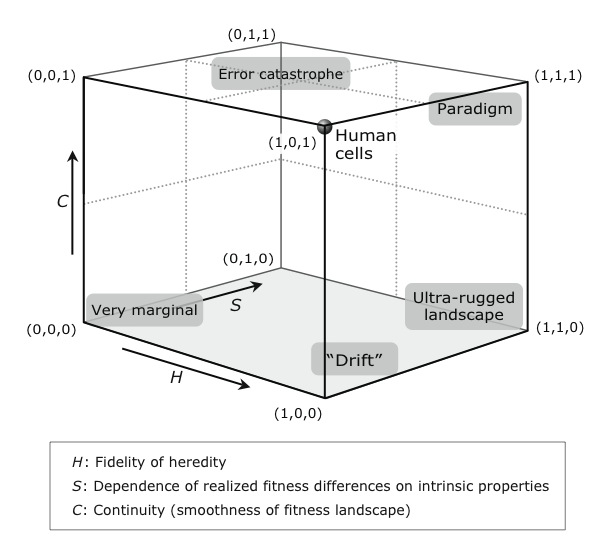
\includegraphics{./images/PGS.png}
	\end{center}
	\caption{L'espace tridimensionnel extrait de \citet[p.~64]{godfrey2009darwinian}}
	\label{fig:PGS}
\end{figure}

Selon l'auteur, cette décomposition des caractéristiques des populations par les différents facteurs qu'il propose n'est pas la seule possible. On pourra trouver d'autres caractéristiques importantes, les décomposer plus finement, ou même décomposer totalement différemment en fonction des besoins.  On pourra mettre en avant certaines caractéristiques pour éclaircir un cas précis et en considérer d'autres comme négligeable, puis inverser les hypothèses et changer la caractéristique centrale à étudier. D'ailleurs, l'auteur illustre la souplesse de cette approche en réfléchissant à ce qu'il appelle les <<\,reproducteurs collectifs\,>>. Pour attaquer l'étude de ces concepts il utilise d'autres caractéristiques qui lui permettent de mieux classer les populations qui correspondent à ces <<\,reproducteurs collectifs\,>>. Dans ces populations, les facteurs que nous avons évoqué précédemment sont déjà plus ou moins clairs et fixés, l'intérêt est déplacé sur d'autres dimensions de l'espace de PGS.

La vision de ce dernier permet donc de rendre compte du monde du vivant d'une façon assez complète:
\begin{quotation}
	Une [vision] dans laquelle les constituants du monde sont un large panel de populations darwiniennes: des cas paradigmatiques et des cas marginaux, certains clairs et d'autres obscurs, certains puissants et d'autre limités. Certains sont visibles et évidents, d'autre sont invisibles. Certains sont à l'intérieur d'autres. Ils avancent selon leur comportement darwinien suivant une large gamme d'échelles différentes, temporelles et spatiales. Certains évoluent via la reproduction d'un tout défini, d'autres évoluent en cooptant le matériel biologique qui en résulte [de la reproduction des premiers]. Les populations évoluent en fonction de leurs propriétés darwiniennes, mais changent aussi la base de leurs évolutions futures, en se déplaçant dans l'espace imaginaires de leurs paramètres évolutifs.\\
	\citep[p.~128]{godfrey2009darwinian}
\end{quotation}

Nous pensons que ce cadre de réflexion est l'outil idéal pour assurer le lien entre la Robotique \'Evolutionnaire et les recherches en Biologie car il permet de réfléchir à des cas d'évolution très différents tout en les situant sur un même continuum. Pour PGS ces cas ne sont pas de nature différente, et diffèrent juste de degré de certaines propriétés. Cela permet de lier entre eux des systèmes à première vue très différents les uns des autres, et de donner d'intéressantes pistes quant au chemin évolutif à suivre pour passer de l'un à l'autre.  Nous verrons comment ce cadre offre un moyen pratique pour positionner les recherches en Robotique et les comparer avec les connaissances des systèmes biologiques, tout en offrant aux chercheurs des indices sur les façons de construire leurs systèmes artificiels.


\section{Conclusion}
Dans cette partie nous avons essayé de montrer comment la théorie de l'évolution, telle que Darwin l'avait imaginée, est structurée et certains problèmes qu'elle a pu et peut encore rencontrer. Pour arriver à cette fin nous avons rapidement retracé l'histoire de cette théorie, en suivant le modèle de \cite{gayon1991darwinetlapresdarwin}. Nous avons notamment parlé des objections faites par Jenkin et comment ces objections ont amené les biologistes à utiliser l'outil statistique pour essayer de manipuler, comprendre et illustrer la théorie de l'évolution. Dans ce but nous avons présenté les travaux des biométriciens, pour ensuite décrire l'état actuel de la théorie en décrivant brièvement la vision la plus largement admise dans la communauté scientifique, amenée par la Synthèse Moderne que nous présentons dans ses (très) grandes lignes.

Nous avons ensuite essayé de montrer quelles pouvaient être aujourd'hui les questions qui agitent ces consensus, en illustrant les problèmes qui ont émergé et qui se sont cristallisés autour du débat sur les unités et niveaux de sélection. Sans nous prétendre exhaustifs, nous avons essayé de dégager quelques positions caractéristiques prises autour de ce débat, puis nous avons terminé en développant le cadre de réflexion de \cite{godfrey2009darwinian} dans lequel nous souhaitons positionner notre objet d'étude principal à savoir: la Robotique \'Evolutionnaire.

Cette mise au point théorique nous semble importante car elle permet \begin{inparaenum}[(\itshape\,1\,\upshape)]
\item de clarifier la théorie que reprennent l'algorithmique et la Robotique \'Evolutionnaire,
\item de souligner les limites et les objectifs de cette théorie,
\item de comprendre avec précision à quelles questions et quels problèmes un outil ayant pour but l'étude de la théorie de l'évolution va rencontrer et doit pouvoir répondre. 
\end{inparaenum}

Avant de décrire (dans la dernière partie) la Robotique \'Evolutionnaire et l'avancer comme un outil d'étude pour explorer cette théorie que nous venons de décrire, nous allons, dans la partie suivante, avancer d'autres outils théoriques et empiriques utilisés par les chercheurs et philosophes pour réfléchir et trouver des réponses aux débats qui remuent la biologie l'évolution tel celui présenté dans la partie \ref{sec:lvl}.
